\documentclass{article}

\usepackage{fancyhdr}
\usepackage{extramarks}
\usepackage{xcolor}
\usepackage{amsmath}
\usepackage{amsthm}
\usepackage{amssymb}
\usepackage{amsfonts}
\usepackage{tikz}
\usepackage[plain]{algorithm}
\usepackage{algpseudocode}
\usepackage[left=1in]{geometry}
\usepackage[shortlabels]{enumitem}
\usepackage{transparent}
\usetikzlibrary{automata,positioning}


%%%%%%%%%%%%%%%%%%%%%%%%%%%%%%%%%%%%%%%%%%%%%%%%%%%%%%%%%%%%%%%%%%%%%%%%%
%%%%%%%%%%%%%%%%%%%%%%%%%%%%% PDF COLOR %%%%%%%%%%%%%%%%%%%%%%%%%%%%%%%%%
%%%%%%%%%%%%%%%%%%%%%%%%%%%%%%%%%%%%%%%%%%%%%%%%%%%%%%%%%%%%%%%%%%%%%%%%%
\usepackage{xcolor} \pagecolor[rgb]{0,0,0} \color[rgb]{0.9,0.9,0.9}
%%%%%%%%%%%%%%%%%%%%%%%%% SUPPRESS UNDERFULL HBOX %%%%%%%%%%%%%%%%%%%%%%%
\hbadness = 20000
%%%%%%%%%%%%%%%%%%%%%%%%%%%%%%%%%%%%%%%%%%%%%%%%%%%%%%%%%%%%%%%%%%%%%%%%%
%
% Basic Document Settings 
%
\topmargin=-0.75in
\evensidemargin=0in
\oddsidemargin=0in
\textwidth=6.5in
\textheight=9.0in
\headsep=0.25in

\linespread{1.1}
\fancypagestyle{plain}{}
\pagestyle{fancy}
\fancyhf{}

\chead{\hmwkClass: \hmwkTitle}
\lfoot{\lastxmark}
\cfoot{\thepage}

\renewcommand\headrulewidth{0.4pt}
\renewcommand\footrulewidth{0.4pt}

\setlength\parindent{0pt}

\newcommand{\bd}{\textbf}
\newcommand{\hmwkTitle}{Homework\ \#2}
\newcommand{\hmwkClass}{Computational Modules}

\newcommand{\nat}{\mathbb{N}}
\newcommand{\lang}{\mathcal{L}}
\newcommand{\AB}{\Sigma}
\newcommand{\ch}{\sigma}
\newcommand{\de}{\delta}
\newcommand{\empw}{\varepsilon}
\newcommand{\ceq}[1]{\overset{#1}{\thicksim}}
\newcommand{\nceq}[1]{\overset{#1}{\nsim}}



% use for comment block, surround block with "\/*" and at the end "*/" 
\long\def\/*#1*/{}


%%%%%%%%%%%%%%%%%%%%%%%%%%%%%%%%%%%%%%%%%%%%%%%%%%%%%%%%%%%%%%%%%%%%%%%%%

\newcommand{\hmwkAuthorName}{\bd{Michael Zhitomirsky}, ID 321962714}

%%%%%%%%%%%%%%%%%%%%%%%%%%%%%%%%%%%%%%%%%%%%%%%%%%%%%%%%%%%%%%%%%%%%%%%%%

%
% Title 
%

\title{
    \textmd{\bd{\hmwkClass:\ \hmwkTitle}}\\
}
\author{\hmwkAuthorName}

\begin{document}

\maketitle

\begin{enumerate}
      \item
            \begin{enumerate}
                  \item 
$\lang''=\{x_1 x_2 . . . x_k : k \in \nat ,x_i \in \AB \text{ for every }
    1 \leq i \leq k \\ \text{ and } \exists y_1,y_2,...y_{2k} \in \AB
    \text { such that } x_1 y_1 y_2 x_2 y_3 y_4...x_k y_{2k-1} y_{2k} \in \lang \}$
\\ \\
We shall construct the following NFA $N''$ for $\lang''$: \\
$N''=(Q, \AB, \de'', S=\{q_0\}, F)$, such that the
transition function is: \\
$\de''(q,\ch)=\{\de(\de(\de(q,\ch),a),b) : \forall a,b \in \AB\},
    \forall q \in Q, \forall \ch \in \AB$. \\
Meaning that $\de''$ is using $\de$ to make one step with $\ch$ and
then 'guess' two steps with all possible symbols in $\AB$.
\\ \\
Now, we shall prove its correctness: \\
We need to show that: $w \in \lang'' \Longleftrightarrow  w \in \lang(N'')$. \\
Note that: \\
$w \in \lang''$\\

(From definition of $\lang''$) \\
$\Longleftrightarrow w \in \{x_1 x_2 . . . x_k : k \in \nat ,x_i \in \AB \text{ for every }
    1 \leq i \leq k \\ \text{ and } \exists y_1,y_2,...y_{2k} \in \AB
    \text { such that } x_1 y_1 y_2 x_2 y_3 y_4...x_k y_{2k-1} y_{2k} \in \lang \}$  \\

(From definition of $A$: $\lang = \lang(A)$) \\
$\Longleftrightarrow \exists k \in \nat ,x_1...x_k \in \AB^*:  w=x_1 x_2 . . . x_k, \\
    \text{ and } \exists y_1,y_2,...y_{2k} \in \AB
    \text { such that } w_{\lang}=x_1 y_1 y_2 x_2 y_3 y_4...x_k y_{2k-1} y_{2k} \in \lang=\lang(A)$ \\

(From definition of $A$) \\
$\Longleftrightarrow \exists q_1,q_2,...q_{3k} \text{ s.t. } $\\
$
    \de(q_0,x_1)=q_1, \de(q_1,y_1)=q_2, \de(q_2,y_2)=q_3, ..., \\
    \de(q_{3k-3},x_{k})=q_{3k-2}, \de(q_{3k-2},y_{2k-1})=q_{3k-1}, \de(q_{3k-1},y_{2k})=q_{3k} \in F
$ \\ \\
(*) Now, from the above and the definition of $\de''$ we get that: \\
$\exists q_1,q_2,...q_{3k} \text{ s.t. } $\\
$
    \de''(q_0,x_1)=\{\de(\de(\de(q_0,x_1),a),b) : \forall a,b \in \AB\} \ni q_3 \text{ } (q_0 \in S), ..., \\
    \de''(q_{3i-3},x_{i})=\{\de(\de(\de(q_{3i-3},x_{i}),a),b) : \forall a,b \in \AB\} \ni q_{3i}, ..., \\
    \de''(q_{3k-3},x_{k})=\{\de(\de(\de(q_{3k-3},x_{k}),a),b) : \forall a,b \in \AB\} \ni q_{3k} \text{ } (q_{3k} \in F)
$ \\ \\

(From definition of $N''$) \\
$\Longleftrightarrow w=x_1 x_2 . . . x_k \in \lang(N'')$ \\
\\
Note that when looking at the proof in the direction of - ($w \in \lang'' \Longleftarrow  w \in \lang(N'')$),
we get transition (*) by choosing  $y_1,y_2,...y_{2k}$ from the specific $a,b \in \AB$ that give us the
accepting branch in the NFA $N''$ for input $w=x_1 x_2 ... x_k$.
\\

In conclusion, we got $w \in \lang'' \Longleftrightarrow  w \in \lang(N'')$. Thus, concluding the proof. \\


                        \pagebreak

                  \item $\lang''=\{xy : yx \in \lang \}$
\\ \\
The idea would be to construct an NFA per state $q \in Q$, $N_q$,
each NFA will check if we can 'break' the word $yx \in \lang$ in state q of $A$.
So each NFA will contain 2 copies of $A - A_{q,1}, A_{q,2}$ such that for
$yx \in \lang$, $x$ will take us from state q in $A_{q,1}$ to $F_{q,1}$
which will be connected with $\empw$-moves to $q_{0,q,2}$ in $A_{q,2}$,
and y will take us from there to state q in $A_{q,2}$.

The main NFA, $N''$, will be a 'union' of the he smaller NFAs ($N_q, \forall q \in Q$).
It will have an initial state group that is the group of the initial states of each of the
smaller NFAs ($N_q, \forall q \in Q$), and that way we will check if word $w$
is some rotation of some word in $\lang$.

Now, we shall give formal definitions for every one of the NFAs: \\

\underline{$\forall q \in Q, N_q$:} \\

$N_q=(Q \times \{1,2\} \times \{q\}, \AB, \de_q, S_q=\{(q, 1, q)\}, F_q=\{(q, 2, q)\})$, \\
such that the transition function is: \\
\[
    \de_q((q', k, q),\ch) = \left.
    \begin{cases}
        \{(\de(q',\ch)\}, k, q)\} , & \ch \in \AB                          \\
        \{(q_0, 2, q)\},            & q' \in F \wedge k=1 \wedge \ch=\empw \\
    \end{cases}
    \right\} , \text{ } k \in \{1,2\}, \ch \in \AB \cup \{\empw\}
\]

\underline{$N''$:} \\

$N''=((Q \times \{1,2\} \times Q), \AB, \de'',
    S''=\{(q_i, 1, q_i) : q_i \in Q\}, F''=\{(q_f, 2, q_f) : q_f \in Q\})$, \\
such that the transition function is: \\
\[
    \de''((q', k, q),\ch) = \de_{q}((q', k, q),\ch),  k \in \{1,2\}, \ch \in \AB \cup \{\empw\}
\]

Now, we shall prove its correctness: \\
We need to show that: $w \in \lang'' \Longleftrightarrow  w \in \lang(N'')$. \\
Note that: \\
$w \in \lang''$\\

(From definition of $\lang''$) \\
$\Longleftrightarrow w \in \{xy : yx \in \lang \}$ \\

(From definition of $A$: $\lang = \lang(A)$) \\
$\Longleftrightarrow \exists x=x_1...x_n,y=y_1...y_m \in \AB^* : w=xy \wedge yx \in \lang = \lang(A)$ \\
\\ \\

(From definition of $A$) \\
$\Longleftrightarrow \exists q_1,q_2,...q_m, q_{m+1}...q_{n+m} \text{ s.t. } $\\
$
    \de(q_0,y_1)=q_1, \de(q_1,y_2)=q_2, ..., \\
    \de(q_{m-1},y_m)=q_m, \de(q_m,x_1)=q_{m+1},...,\\
    \de(q_{n+m-1},x_{n})=q_{n+m} \in F
$ \\

(From definition of $\de''$) \\
$\Longleftrightarrow \exists q_1,q_2,...q_m, q_{m+1}...q_{n+m} \text{ s.t. } $\\
$
    \de''((q_m, 1, q_m), x_1) \ni (q_{m+1}, 1, q_m) \text{ } ((q_m, 1, q_m) \in S''), ..., \\
    \de''((q_{n+m-1}, 1, q_m), x_n) \ni (q_{n+m}, 1, q_m),\\
    \de''((q_{n+m}, 1, q_m), \empw) \ni (q_0, 2, q_m), (q_{n+m} \in F)\\
    \de''((q_0, 2, q_m), y_1) \ni (q_1, 2, q_m), ...,\\
    \de''((q_{m-1}, 2, q_m), y_m) \ni (q_m, 2, q_m) \text{ } ((q_m, 2, q_m) \in F'')
$ \\

(From definition of $N''$) \\
$\Longleftrightarrow w=x_1...x_n y_1... y_m \in \lang(N'')$ \\

All in all, we got $w \in \lang'' \Longleftrightarrow  w \in \lang(N'')$. Thus, concluding the proof. \\

            \end{enumerate}

            \pagebreak

      \item Formally describe a 2-tape non-deterministic TM that on input $\#1^n\#$ such
that $n > 1$ chooses non-deterministically $i, j$ such that $0 < i, j \leq n$, writes
$1^i\#1^j$ on the second tape and accepts. You may use a model that allows the
head to stay put (S) as well as moving right (R) and left (L). \\

We will denote the required TM by $M$. \\
The formal description of $M$ will be: \\
$ M = (Q, \AB, \Gamma, \de, q_0, q_a, q_r) $ such that: \\
$ Q      = \{q_0, q_i, q_j, q_a, q_r\} $ \\
$ \AB    = \{1, \#\} $ \\
$ \Gamma = \AB \cup \{\sqcup\} $ \\
and $\de$ is defined by:

\begin{figure}[h]
    \centering
    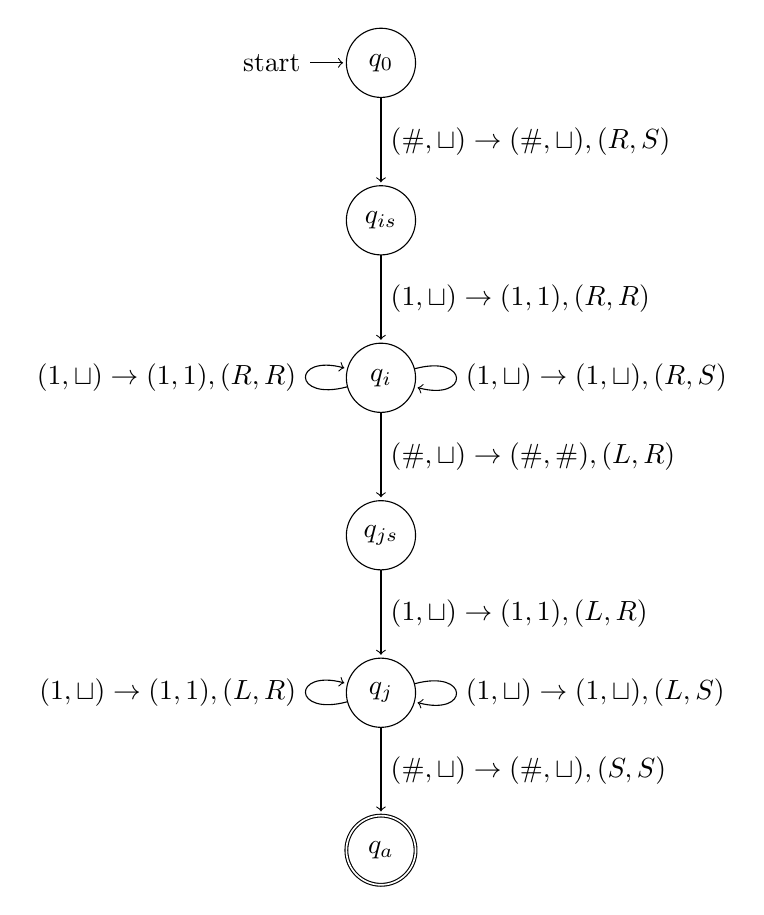
\begin{tikzpicture}[shorten >=1pt,node distance=2cm,on grid,auto]
        \node[state, initial]   (q_0)                  {$q_0$};
        \node[state]            (q_is) [below=of q_0]  {$q_{is}$};
        \node[state]            (q_i)  [below=of q_is] {$q_i$};
        \node[state]            (q_js) [below=of q_i]  {$q_{js}$};
        \node[state]            (q_j)  [below=of q_js] {$q_j$};
        \node[state, accepting] (q_a)  [below=of q_j]  {$q_a$};

        \path[->]
        (q_0)
        edge              node {$(\#, \sqcup) \rightarrow (\#,\sqcup), (R,S)$} (q_is)

        (q_is)
        edge              node {$(1, \sqcup)  \rightarrow (1,1),       (R,R)$} (q_i)

        (q_i)
        edge [loop left]  node {$(1, \sqcup)  \rightarrow (1,1),       (R,R)$} (q_i)
        edge [loop right] node {$(1, \sqcup)  \rightarrow (1, \sqcup), (R,S)$} (q_i)
        edge              node {$(\#, \sqcup) \rightarrow (\#,\#),     (L,R)$} (q_js)

        (q_js)
        edge              node {$(1, \sqcup)  \rightarrow (1,1),       (L,R)$} (q_j)

        (q_j)
        edge [loop left]  node {$(1, \sqcup)  \rightarrow (1,1),       (L,R)$} (q_j)
        edge [loop right] node {$(1, \sqcup)  \rightarrow (1, \sqcup), (L,S)$} (q_j)
        edge              node {$(\#, \sqcup) \rightarrow (\#,\sqcup), (S,S)$} (q_a);

    \end{tikzpicture}
    \label{fig:multiple5}
\end{figure}


Short explanation: \\
1. First we go over the input from left to right and each time we see '1' we choose
to write '1' on the second tape or write nothing and move on.

2. When we reach the end of the input we have written the '$1^i$' part on the second tape, so we write '$\#$'.

3. Then we go over the input from right to left and repeat the process - each time we
see '1' we choose to write '1' on the second tape or write nothing and move on.

4. When we reach the beginning of the tape, at that point we have written '$1^i\#1^j$' on the second tape,
where $i, j$ were chosen non-deterministically.


            \pagebreak

      \item Prove / Disprove:
            \begin{enumerate}
                  \item If $\lang_1, \lang_2 \in \Pcl$ are non-trivial ($\lang_1, \lang_2 \notin \{\emptyset, \AB^*\}$), then there exists a polynomial shrinking
reduction from $\lang_1$ to $\lang_2$.
                  \item If $\lang_1, \lang_2 \in \NPcl$ are non-trivial ($\lang_1, \lang_2 \notin \{\emptyset, \AB^*\}$), then there exists a polynomial shrinking
reduction from $\lang_1$ to $\lang_2$.


if there is reduction then whole NP is NPC, beacuse P is NP we get P in NPC, then P=NP=NPC
                        \pagebreak

                  \item $\lang=\{w : \exists n \in \nat \text{ s.t. } |w| = n^3\}$
(twice, once using the pumping lemma and once using Myhill-Nerode)

\underline{Using Pumping Lemma} \\

We will prove by contradiction - we will assume that $\lang$ is regular.
Since $\lang$ is regular, we can apply the pumping lemma to $\lang$. Let $k$
be the number from the pumping lemma for $\lang$. We will choose $w = 0^{3^k}$.
Note that $|w|=3^k \rightarrow w \in \lang \text{ and } |w| \geq k$.
Therefore, from the pumping lemma, there exists some $x, y, z$ where $w = xyz$ and:

\begin{enumerate}
    \item $\forall i \geq 0: x y^i z \in \lang$
    \item $|y| > 0$
    \item $|xy| \leq k$
\end{enumerate}

From (ii) and (iii) we get that $y=0^j, 0 < j \leq k$,
note that $x y^2 z = 0^{k^3} 0^j = 0^{k^3+j}$,
so we get
\[
    |x y^2 z| = k^3+j
\]
but
\[
    k = \sqrt[3]{k^3} < \boldsymbol{\sqrt[3]{k^3+j}} < \sqrt[3]{k^3+k} < \sqrt[3]{k^3+3k^2+3k+1} = \sqrt[3]{(k+1)^3} = k+1
\]
so $\sqrt[3]{k^3+j} \notin \nat$, meaning $x y^2 z \notin \lang$ in contradiction with (i). \\
We got a contradiction, hence $\lang$ is not regular. \\


\underline{Using Myhill-Nerode Theorem} \\

Note that for $i < j$ we get $x = 0^{i^3+1} \nceq{\lang} 0^{j^3+1}  = y$,
since for $z=0^{3i^2+3i} \in \AB^*$ we get:

$xz = 0^{i^3+1}0^{3i^2+3i}=0^{i^3+3i^2+3i+1}=0^{(i+1)^3} \in \lang \text{ } (\sqrt[3]{|xz|}=\sqrt[3]{(i+1)^3}=i+1 \in \nat$, \\
but $yz = 0^{j^3+1}0^{3i^2+3i}=0^{j^3+3i^2+3i+1}$, so:
\[
    |yz| = j^3+3i^2+3i+1
\]
and
\[
    j = \sqrt[3]{j^3} < \boldsymbol{\sqrt[3]{j^3+3i^2+3i+1}} < \sqrt[3]{j^3+3j^2+3j+1} = \sqrt[3]{(j+1)^3} = j+1
\]
so $\sqrt[3]{j^3+3i^2+3i+1} \notin \nat$, meaning $yz \notin \lang$.

Hence, each $ 0^{i^3+1} $ belongs to a different equivalence class for every $i \geq 0$, \\
meaning $|\AB^* / \ceq{\lang}| \geq |\{0^{i^3+1}: i \geq 0\}| = \infty$ \\
We got that $\lang$ has an infinite number of equivalence classes, hence from
Myhill-Nerode Theorem we get that $\lang$ is not regular. \\
                        \pagebreak

                  \item Let us define $Prefix(\lang) = \{x : \exists y \text{ such that } xy \in \lang\}$

\begin{enumerate}[i.]
    \item $\REcl$ is closed under Prefix.

          The claim is true. \\

          Proof: \\
          Let there be $\lang \in \REcl$, we will show that $Prefix(\lang) \in \REcl$. \\
          $\lang \in \REcl$ so there is TM $M$ that accepts $\lang$. \\
          We shall build a non-deterministic TM $N$ that accepts $Prefix(\lang)$:

          $N \text{ on input } x$: \\
          1. order $\AB^*$ in a lexicographic order. \\
          2. for each word $y$ in that order, run $M$ on $w=xy$ in parallel. \\
          3. accept iff $M$ accepts for some word $w=xy$. \\

          Note - instead of using a non-deterministic TM, we can run $M$ on each of \\
          the words in 'parallel' by running each time on an increasing number of \\
          words for an increasing number of steps, just like we did in the lecture and recitation. \\ \\ \\ \\ \\ \\


          \TODO
          So we get: \\
          if $x \in Prefix(\lang)$ then
          $\exists y \in \AB^*: w=xy \in \lang \rightarrow $ in one of the computational
          paths for input $x$, $N$ will choose $y$ for $x$ and $M$ would accept $w=xy \in \lang$
          $\rightarrow N$ accepts. \\

          if $x \notin \lang^*$  then
          $\nexists x_1,...,x_n \in \lang: x=x_1...x_n \rightarrow $ there is no computational
          path for input $x$, in which $N$ will choose a split such that $M$ would accepts all of its parts.
          But, because $M$ decides $\lang$ we will get that $M$ will reject at least one of the parts in
          each of the arbitrary splits and accept the others and wouldn't be stuck in a loop $\rightarrow N$ rejects. \\

          Indeed we get that $N$ decides $\lang^*$. \\
          So we get that  $\Rcl$ is closed under Kleene star, as required. \\



    \item $\Rcl$ is closed under Prefix.


\end{enumerate}
                        \pagebreak

                  \item Let us define $LHS(\lang) = \{x : \exists y \text{ such that } xy \in \lang\ \text{ and } |x| = |y|\}$

\begin{enumerate}[i.]
      \item $\REcl$ is closed under LHS.

            The claim is true. \\

            Proof: \\
            Let there be $\lang \in \REcl$, we will show that $LHS(\lang) \in \REcl$. \\
            $\lang \in \REcl$ so there is TM $M$ that accepts $\lang$. \\
            We shall build a non-deterministic TM $N$ that accepts $LHS(\lang)$:

            $N \text{ on input } x$: \\
            1. Order $\AB^{|x|}$ in a lexicographic order. \\
            2. For each word $y$ in that order, run $M$ on $w=xy$ in parallel. \\
            3. Accept iff $M$ accepts for some word $w=xy$. \\

            Note - instead of using a non-deterministic TM, we can run $M$ on each of \\
            the words in 'parallel' by running each time on an increasing number of \\
            words for an increasing number of steps, just like we did in the lecture and recitation. \\

            So we get: \\
            If $x \in LHS(\lang)$ then: \\
            $\exists y \in \AB^{|x|}: w=xy \in \lang \rightarrow $ in one of the computational
            paths for input $x$, $N$ will choose $y$ for input $x$ and $M$ would accept $w=xy$. \\
            $\rightarrow N$ accepts. \\

            If $x \notin LHS(\lang)$ then: \\
            $\nexists y \in \AB^{|x|}: w=xy \in \lang \rightarrow $ there is no computational
            path for input $x$, in which $N$ will choose $y$ such that $w=xy \in \lang$,
            so $M$ would reject or be stuck in a loop for every $w=xy$. \\
            $\rightarrow N$ rejects or stuck in a loop. \\

            Indeed we get that $N$ accepts $LHS(\lang)$. \\
            So we get that $\REcl$ is closed under LHS, as required. \\

      \item $\Rcl$ is closed under LHS.

            The claim is true. \\

            Proof: \\
            Let there be $\lang \in \Rcl$, we will show that $LHS(\lang) \in \Rcl$. \\
            $\lang \in \Rcl$ so there is TM $M$ that decides $\lang$. \\
            We shall build a deterministic TM $M'$ that decides $LHS(\lang)$:

            $M' \text{ on input } x$: \\
            1. Order $\AB^{|x|}$ in a lexicographic order. \\
            2. For each word $y$ in that order, run $M$ on $w=xy$. \\
            3. Accept iff $M$ accepts for some word $w=xy$. \\

            So we get: \\
            If $x \in LHS(\lang)$ then: \\
            $\exists y \in \AB^{|x|}: w=xy \in \lang \rightarrow $ at some point, $M$ would run on $w=xy$ and accept it. \\
            $\rightarrow M'$ accepts. \\ \\

            If $x \notin LHS(\lang)$ then: \\
            $\nexists y \in \AB^{|x|}: w=xy \in \lang \rightarrow $ $M$ would reject $w=xy$ for every $y \in \AB^{|x|}$. \\
            $\rightarrow M'$ rejects. \\

            Notice that $M$ doesn't get stuck in a loop for any $w=xy$ because it decides $\lang$.
            Also there is a finite amount of extensions $y$ for $x$ ($=|\AB|^{|x|}$).
            Therefore $M'$ doesn't get stuck in a loop. \\

            Indeed we get that $M'$ accepts $LHS(\lang)$. \\
            So we get that $\Rcl$ is closed under LHS, as required. \\

\end{enumerate}
            \end{enumerate}

            \pagebreak

      \item A function $f : \AB^* \rightarrow \AB^*$ is computable if there exists a TM that for every
            $x \in \AB^*$ halts with $f(x)$ on its tape, when given $x$ as input.
            Let $f : \AB^* \rightarrow \AB^*$ be a function, then let us define $\lang_f = {(x, f(x)) : x \in \AB^*}$
            \begin{enumerate}
                  \item polynomial verifier runtime is at most $p(|x|)$, hence it would not look beyond the first $p(|x|)$ symbols of $w$,
hence $w$ can be of length at most $p(|x|)$.
If the length of $w$ is less than $p(|x|)$, then we can pad $w$ until its length reaches exactly $p(|x|)$
In conlusion there is a verifier for $\lang$ that only accepts cerificates of length exactly $p(|x|)$
(its behaviour would be identical to the behaviour of the standard verifier with the addional check
that the length of the cerificate it receives as input is exactly $p(|x|)$, if it is not - it rejects.)

***build the verfier***
                  \item Prove that $CIRSAT \in \NPCcl$ (use ”the heart of Cook-Levin” from Lecture 10).  \\

Proof: \\
We need to show that: \\
1. $CIRSAT \in NP$ \\
2. $\forall \lang \in \NPcl: \lang \leq_p CIRSAT$ \\

First we show that $CIRSAT \in NP$, by building a polynomial verifier $V$ for it. \\
$V$ for input $(\langle C, x \rangle, w)$:
\begin{enumerate}[1., itemsep=5pt]
    \item Verify that $\langle C, x \rangle$ is a valid encoding of a boolean circuit and a partial input, if it's not - reject.

    \item Calculate $C(xw)$

    \item If $C(xw)=1$ - accept, otherwise - reject.

\end{enumerate}

Indeed: \\
If $\langle C, x \rangle \in CIRSAT$ \\
$\Rightarrow \langle C, x \rangle$ is a valid encoding of boolean circuit and a partial input
and there exists $w \in \AB^*$ such that $C(xw)=1$. \\
$\Rightarrow $ There exists $w \in \AB^*$ such that $V$ accepts $(\langle C, x \rangle, w)$. \\

If $\langle C, x \rangle \notin CIRSAT$ \\
$\Rightarrow \langle \phi \rangle$ is not a valid encoding of a boolean circuit and a partial input
or there doesn't exist $w \in \AB^*$ such that $C(xw)=1$. \\
If $\langle C, x \rangle$ is not a valid encoding of a boolean circuit and a partial input $\Rightarrow V$ rejects. \\
If there doesn't exist $w \in \AB^*$ such that $C(xw)=1$ \\
$\Rightarrow V$ rejects $(\langle C, x \rangle, w)$ for every $w \in \AB^*$.

Also $V$'s runtime on input $(\langle C, x \rangle, w)$ (where $|\langle C, x \rangle|=n$) is: \\
- For step (1): $O(q(n))$ for some polynomial function $q$ \\
- For step (2): $O(k(n))$ for some polynomial function $k$ \\
- For step (3): $O(1)$ \\
Thus, the total runtime of $V$ on input  $(\langle C, x \rangle, w)$ is polynomial in $|\langle C, x \rangle|=n$, so \underline{$CIRSAT \in \NPcl$}. \\

\pagebreak

Now we show that $\forall \lang \in \NPcl: \lang \leq_p CIRSAT$ \\
Let there be $\lang \in \NPcl$, therefore there exists a polynomial verifier $V_\lang$ for $\lang$, that only accepts
certificates of length exactly $p(|x|)$, where $p$ is the polynomial runtime of the verifier (we get this from the previuos section). \\

From ”the heart of Cook-Levin” in Lecture 10, for a TM $M$ that runs in time $t(n)$
there exists a function that is computable in time $g(t(n))$ (where $g$ is a polynomial function), that given $1^n$ as input, calculates
the encoding of a boolean circuit $C_{M,n}: \{0,1\}^n \rightarrow \{0,1\}$
such that: \\
1. $\forall z \in \{0,1\}^n: M(z)$ accepts $\iff C_{M,n}(z)=1$ \\
2. $|C_{M,n}| \leq O(t^2(n))$ \\

We denote the function that calculates the encoding of the boolean circuit in ”the heart of Cook-Levin” by $f$. \\
We will use the verifier $V_\lang$ as the TM in ”the heart of Cook-Levin”.

Now we will show that there is a polynomial reduction from $\lang$ to $CIRSAT$: \\
We define the following reduction $h: \AB^* \rightarrow \AB^*$:
$h(x) = (\langle f(1^{|x|+p(|x|)}), x \rangle)$

Notice that $h$ is computable in polynomial time, since it takes $O(g(p(n+p(n))))$ (where $|x|=n$ and $g$, $p$ are polynomial functions)
to calculate $f(1^{|x|+p(|x|)})$.

Also $\forall x \in \AB^*$:

If $x \in \lang$ \\
$\Rightarrow $ There exists $w \in \AB^{p(|x|)}$ such that $V_\lang$ accepts $(x, w)$. \\
$\Rightarrow $ From (1) of ”the heart of Cook-Levin”, for $h(x) = (\langle f(1^{|x|+p(|x|)}), x \rangle) = (\langle C, x \rangle)$,
we get $C(xw)=1$ \\
$\Rightarrow h(x) = (\langle f(1^{|x|+p(|x|)}), x \rangle) \in CIRSAT$ \\

If $x \notin \lang$ \\
$\Rightarrow V$ rejects $(x, w)$ for every $w \in \AB^*$. \\
$\Rightarrow $ From (1) of ”the heart of Cook-Levin”, for $h(x) = (\langle f(1^{|x|+p(|x|)}), x \rangle) = (\langle C, x \rangle)$,
we get $C(xw)=0$ for every $w \in \AB^{p(|x|)}$ \\
$\Rightarrow h(x) = (\langle f(1^{|x|+p(|x|)}), x \rangle) \notin CIRSAT$ \\

So we get \underline{$\lang \leq_p CIRSAT$}. \\
In conclusion, $CIRSAT \in \NPCcl$. As required.

            \end{enumerate}

            \pagebreak

      \item Let us define: \\ \\
$
    \begin{aligned}
        Size(O(1)) = \{ & \lang : \text{ There exists a circuit ensemble } C=\{C_n\}_{n \in \nat} \\
                        & \text{such that } \lang(C)=\lang \text{ and } |C_n|\in O(1\}
    \end{aligned}
$ \\ \\
We will present a non-regular $\lang$ such that $\lang \in Size(O(1))$.

We will use the language in question 3c: \\
$\lang=\{w : \exists n \in \nat \text{ s.t. } |w| = n^3\}$ \\
it was proven in 3c that the above language is not regular.

We can construct the following circuit ensemble $C=\{C_n\}_{n \in \nat}$ \\
such that $\lang(C)=\lang$ and $|C_n|\in O(1\}$:

if $n$ is a cube of an integer ($\sqrt[3]{n} \in \nat$), then the circuit, $C_n$, will return the constant 1, \\
otherwise (if $\sqrt[3]{n} \notin \nat$) the circuit, $C_n$, will return the constant 0.

Presenting the above as formula:
$
    C_n(x_1 ... x_n) =
    \begin{cases}
        1 , & \sqrt[3]{n} \in \nat    \\
        0 , & \sqrt[3]{n} \notin \nat \\
    \end{cases}
$

Presenting as a diagram: \\
\textcolor{red}
{
    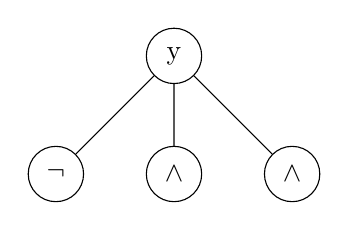
\begin{tikzpicture}[
            every node/.style = {minimum width = 2em, draw, circle},
        ]
        \node {y}
        child {node {$\neg$}}
        child {node {$\wedge$}}
        child {node {$\wedge$}};
    \end{tikzpicture}
}

Indeed, $w \in \lang$ iff then $C_{|w|}(w)=1$.
Therefore $\lang(C)=\lang$ and for each circuit in the ensemble $|C_n| = 0 \in O(1\}$ since there are no logic
gates in all the circuits in the ensemble.

\end{enumerate}

\end{document}